\scanpage{20}

Questions ouvertes

1) Soit $A$ algèbre locale noethérienne sur $k$. Est-il vrai
que $A$ form$^t$ simple sur $k$ si $A$ est univ$^t$ régulière
sur $k$ [i.e., pour hom local $A\longrightarrow B$ d'anneaux
locaux noethériens, équivalence entre ``f$^t$ simple''
et ``univ. régulière'' \deleted{\unsure{sur}} sur $A$].

\margin{\unsure{OK}}

2) Soit $A$ algèbre locale noethérienne sur $k$, f$^t$
simple sur $k$ (pour sa topologie habituelle).
Est-il vrai que $A$ est f$^t$ simple pour sa topologie
discrète? \unsure{Cas où} $A$ est complet ? (Il est
possible que la réponse soit affirmative en
car $p>0$, négative en car 0). -- On peut
généraliser \unsure{au cas où on}. $A$ plat sur $\Lambda$,
\inserted{$A$ et} $\Lambda$ anneaux noethériens: si les
\unsure{localisés} de $A$ sont f$^t$ simples sur ceux de $\Lambda$
pour leur topologie habituelle, $A$ est-il f$^t$.
simple sur $\Lambda$ pour sa top. discrète.

\margin{Faux ! \unsure{valuation}
\uline{\unsure{vrai;}} \uline{\unsure{possibilité}}
Peut-être \unsure{y a-t-il} \unsure{de l'espoir} \unsure{si on}
\unsure{on passe aux} extensions de $B$ \unsure{h.}
\deleted{\unsure{qui}} \unsure{qui sont}
en \unsure{anneaux} \uline{$\unsure{VA}$}
\unsure{(anneaux} à \unsure{résidu fini}).
\unsure{pas} \unsure{universelle} en \unsure{type fini}.}
\margin{\figure{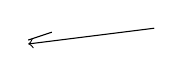
\begin{tikzpicture}\draw[->] (1.6,.2)--(0,0);\draw (0,.05)--(.3,.15);\end{tikzpicture}}}

3) $B$ \deleted{\unsure{libre}} \inserted{plat.} sur $A$, $A$ et $B$ noethériens.
Lieu des $\unsure{p}$ de $\operatorname{Spec}B$ dont l'anneau
local dans la fibre sur $\operatorname{Spec}A$ est f$^t$ simple
sur le corps résiduel en $A$, est-il ouvert?
\deleted{[NB. \unsure{Même}} (Si $B$ n'est pas plat sur $A$,

\mspage{19}
